
    \chapter{Metodologia da Pesquisa}

    Este trabalho se inicia em uma revisão das literaturas, com o uso de diferentes trabalhos publicados em livros, revistas, periódicos e outros, para que sirva de base para suas análises. Por seguinte foram realizadas etapas do ciclo de vida da engenharia de requisitos a fim de se obter um modelo de segurança específico para aplicações bancárias no Android.

    Na Fig \ref{metodologia} mostraremos as etapas de como executaremos a apresentação do modelo proposto. Cada etapa será discutida em detalhes, evidenciando procedimentos realizados e as técnicas implementadas para garantir a integridade, confidencialidade e disponibilidade das informações no ambiente bancário.

    \begin{figure}[H]
    \centering 
    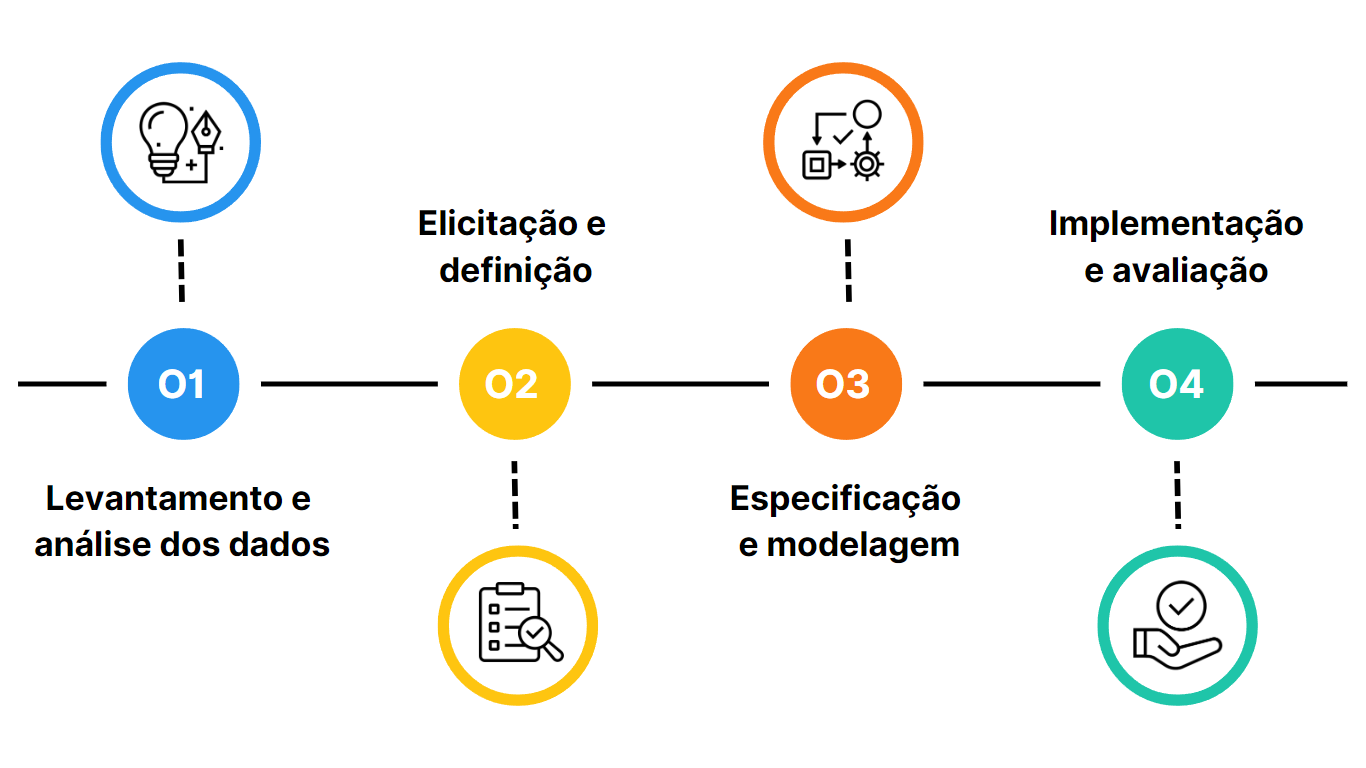
\includegraphics[width = 16cm]{Imagens/metodologia.png}
    \caption{Etapas adotada no trabalho}
    \label{metodologia}
    \end{figure}

    
    \section{Levantamento e análise de dados}
    Para a confecção do presente trabalho foram utilizados artigos científicos encontrados em plataformas públicas como Google Scholar, IEEE Xplore e Typeset.io por meio das palavras chave ``Mobile Banking Security'' e com a data da publicação entre os anos de 2019 e 2024. Como questões da pesquisa foram escolhidas as seguintes perguntas:

    \begin{itemize}[topsep=3pt, partopsep=3pt, itemsep=3pt, parsep=3pt]
        \item Quais são as ameaças de segurança mais críticas do setor bancário no android? 
        \item Quais são os métodos de segurança mais eficazes e viáveis para combater essas ameaças?
    \end{itemize}
    
    Com isso, foram selecionados artigos científicos com conteúdo técnico voltado ao pesquisador e desenvolvedor de aplicações bancárias com foco em segurança da informação, publicados em língua inglesa e com texto completo disponível. Dessa forma, evitando artigos não relacionados ao tema, incompletos, não publicados em língua inglesa e com conteúdo não técnico, isso é, artigos para usuários. Por fim, optou-se por incluir apenas artigos que ajudariam a responder as questão de pesquisa com base em uma leitura exploratória e análise de seu título, palavras-chave e resumo.

    Após a coleta dos dados, procedeu-se à leitura analítica do material, chegando na compilação das informações mais relevantes. Em seguida, foi conduzida uma análise descritiva, que visou não apenas compreender, mas também aprofundar o conhecimento sobre o tema investigado. Essa análise permitiu identificar padrões e tendências nos dados, contribuindo para a construção de um referencial teórico robusto e fundamentado, essencial para a compreensão aprofundada da segurança em aplicações bancárias móveis.

    \section{Elicitação e definição de requisitos de segurança utilizando a técnicas de casos de uso indevido}
    Com o compilado de informações, foi feita a elicitação dos requisitos utilizando a técnica de caso de uso indevido visando entender e descrever as principais interações maliciosas que podem comprometer o sistema e criar uma base para a definição dos requisitos de segurança.
    
    A técnica de casos de uso indevido é uma abordagem que pode ser utilizada na elicitação de requisitos de segurança ao identificar potenciais ameaças e vulnerabilidades que podem comprometer um sistema. Diferente dos casos de uso tradicionais, que descrevem interações desejadas entre usuários e o sistema, os casos de uso indevido focam em interações maliciosas que podem ser realizadas por atacantes para explorar fraquezas no sistema, isto é, as ameaças.

    Com a identificação dos casos de uso indevidos do sistema durante a revisão de literatura, foram definidos requisitos de segurança que especificam controles e mecanismos necessários para mitigar os riscos associados.

    \section{Especificação e modelagem dos requisitos de segurança utilizando diagramas UML}
    Após a elicitação dos requisitos de segurança, foi realizada a especificação e modelagem desses requisitos utilizando diagramas Unified Modeling Language (UML), para representar, organizar e comunicar os aspectos estruturais (estáticos) e comportamentais (dinâmicos) de um sistema de maneira clara e estruturada.

    Para este trabalho, utilizamos o software Visual Paradigm para criar diversos tipos de diagramas UML, incluindo:

    \begin{itemize}[topsep=3pt, partopsep=3pt, itemsep=3pt, parsep=3pt]
        \item Diagramas de Caso de Uso: Representam as interações entre os atores (usuários e sistemas externos) e o sistema, incluindo os casos de uso indevido identificados na fase anterior.
        \item Diagramas de Classe: Mostram como são implementadas as classes dentro do sistema, destacando os pontos onde os requisitos de segurança devem ser aplicados.
        \item Diagramas de Sequência: Ilustram a sequência de mensagens trocadas ou ações realizadas entre os componentes do sistema para cumprir os requisitos de segurança. 
    \end{itemize}
    
    Esses diagramas ajudam a visualizar como os requisitos de segurança se integram com os outros requisitos funcionais do sistema e a identificar possíveis inconsistências ou lacunas. A modelagem também facilita a comunicação e garante um entendimento comum dos requisitos de segurança.

    \section{Estudo de caso e avaliação do modelo}
    A etapa final do processo é um estudo de caso no qual os requisitos de segurança são propostos no ambiente Android, utilizando a aplicação bancária Herd Financial como base. O estudo de caso envolve a demonstração dos casos de uso do modelo de requisitos na aplicação bancária controlada. 

    Este estudo de caso permitiu validar a viabilidade técnica dos requisitos de segurança e testar sua eficácia em um cenário realista. Ao propor medidas de segurança diretamente à aplicação Herd Financial, foi possível observar como os controles de segurança poderiam interagir e se complementar no contexto de uma aplicação bancária. Além disso, este processo forneceu exemplos práticos de como os controles de segurança podem ser incorporados ao código-fonte do aplicativo Android, oferecendo uma referência valiosa para desenvolvedores que buscam implementar práticas de segurança semelhantes em suas próprias aplicações.

    Além disso, uma avaliação detalhada do modelo de segurança proposto para aplicações bancárias no Android, utilizando como referência a certificação PCI DSS. Esta certificação, desenvolvida pela PCI Security Standards Council, é amplamente reconhecida e exigida pelas principais bandeiras de cartão de crédito. A conformidade com os 12 requisitos fundamentais do PCI DSS é crucial não apenas para atender às exigências das organizações de pagamento, mas também para minimizar riscos e fortalecer a confiança dos consumidores na segurança das transações financeiras.

    Este processo de avaliação serve como uma validação técnica da eficácia e da adequação do modelo de segurança no contexto específico de aplicações bancárias no Android. Ao mapear os requisitos do PCI DSS ao modelo proposto, é possível identificar pontos fortes e lacunas, oferecendo insights valiosos para aprimoramento. 
    
    A avaliação do modelo de segurança à luz dos requisitos do PCI DSS e o estudo de caso na aplicação Herd Financial não apenas garantem que as medidas de segurança sejam tecnicamente viáveis, mas também que sejam diretamente aplicáveis e eficazes no contexto específico das aplicações bancárias móveis.
    